\documentclass{standalone}
\usepackage{tikz}
\usepackage{ctex,siunitx}
\setCJKmainfont{Noto Serif CJK SC}
\usepackage{tkz-euclide}
\usepackage{amsmath}
\usetikzlibrary{patterns, calc,3d}
\usetikzlibrary {decorations.pathmorphing,decorations.pathreplacing,decorations.shapes}
\begin{document}
\small
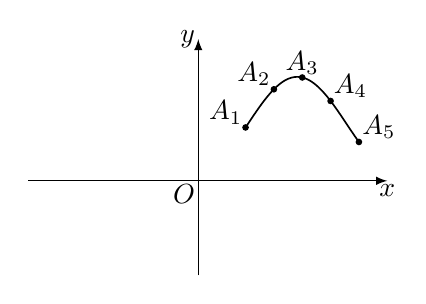
\begin{tikzpicture}[>=latex,scale=1.2,inner sep=1pt]
  \draw[->](-1.8,0)--(2,0)node[below]{$x$};
  \draw[->](0,-1.0)--(0,1.5)node[left]{$y$};
  \node at (0,0)[below left]{$O$};
  \draw[semithick,samples=200,domain=0.5:1.7]plot(\x,{0.6-0.5*cos(3*\x r)});
  \foreach \x/\y[count=\i] in {0.5/above left,0.8/above left,1.1/above,1.4/above right,1.7/above right}
  {
    \fill(\x,{0.6-0.5*cos(3*\x r)})circle(1pt)node[\y]{$A_\i$};
  }
\end{tikzpicture}
\end{document}